\documentclass{book}

\usepackage[a4paper]{geometry}
\usepackage[utf8]{inputenc}
\usepackage{emptypage}
\usepackage{epigraph}
\usepackage{mathtools}
\usepackage{amssymb}
\usepackage{amsthm}
\usepackage{braket}
\usepackage{graphicx}
\usepackage[hidelinks]{hyperref}

\graphicspath{{images/}}

\hypersetup{
	pdftitle={On the Turing Completeness of Recurrent Neural Networks},
	pdfauthor={Francesco Ballerini}
}

\newcommand{\defeq}{\vcentcolon=}
\newcommand{\eqdef}{=\vcentcolon}
\newcommand{\pushone}{\texttt{\textsc{push}}\textsubscript{\texttt{1}}}
\newcommand{\pushzero}{\texttt{\textsc{push}}\textsubscript{\texttt{0}}}
\newcommand{\nonempty}{\textsc{\texttt{nonempty}}}
\newcommand{\tos}{\textsc{\texttt{top}}}
\newcommand{\pop}{\textsc{\texttt{pop}}}
\newcommand{\noop}{\textsc{\texttt{nooperation}}}
\newcommand{\Q}{\mathbb{Q}}
\newcommand{\h}{\mathrm{h}}
\renewcommand{\arraystretch}{1.3}

\theoremstyle{definition}
\newtheorem{definition}{Definition}[chapter]

\theoremstyle{plain}
\newtheorem{theorem}{Theorem}[chapter]
\newcounter{theoremCounter}

\theoremstyle{plain}
\newtheorem{lemma}[theorem]{Lemma}

\theoremstyle{remark}
\newtheorem{remark}{Remark}[theorem]

\theoremstyle{plain}
\newtheorem{corollary}{Corollary}[theorem]

\begin{document}
	
	\frontmatter

	\begin{titlepage}
		\begin{center}
			\vspace*{1cm}
			
			\Huge
			\textbf{On the Turing Completeness of Recurrent Neural Networks}
			
			\vfill
			
			\huge
			\textbf{Francesco Ballerini}
			
			\vfill
			
			\LARGE
			Tesi di Laurea Triennale in Ingegneria Informatica
			
			\vspace{0.5cm}
			
			\Large
			Relatore: Andrew David Bagdanov
			
			\vfill
			
			\includegraphics[width=0.5\textwidth]{logo.pdf}
			
			\vfill
			
			\large
			Università degli Studi di Firenze\\
			Scuola di Ingegneria\\
			a.a. 2018--2019
		\end{center}
	\end{titlepage}
	
	\thispagestyle{empty}\mbox{}\clearpage
	
	\thispagestyle{empty}
	\epigraph{In the end, we self-perceiving, self-inventing, locked-in mirages are little miracles of self-reference.}
		{\textit{I Am a Strange Loop}\\Douglas Hofstadter}
	%\epigraph{The question of whether a computer can think is no more interesting than the question of whether a submarine can swim.}
		%{Edsger Wybe Dijkstra}
	%\epigraph{But can we do more? Can we use PowerPoint to edit images? Yes we can. Can we use PowerPoint to produce videos? You're watching one. Can we use PowerPoint to typeset research papers? With much effort. Can we use PowerPoint to \ldots\ do everything?}
		%{\textit{On the Turing Completeness \\of PowerPoint}\\Tom Wildenhain}
	
	\chapter*{Abstract}
	The purpose of this thesis is to discuss the Turing completeness of recurrent neural networks, which we will model as multilayer feed-forward neural networks feeding their output back into their own input until certain conditions on the output layer are satisfied. In particular, we will prove that, given any binary single-tape Turing machine (actually, any pushdown automaton with two binary stacks) $\mathcal{M}$, it is possible to build a recurrent neural network $\mathcal{N}$ with rational weights, biases, and activations which simulates $\mathcal{M}$: every output generation of $\mathcal{N}$ will correspond to a step in the execution of $\mathcal{M}$. This proof, heavily based on \cite{SiegSon}, will be constructive, yet, due to its generality, very laborious to apply to any given machine; for this reason, we will then show how to deploy its  main ideas in a specific example, also providing an implementation in order to verify, at least in that particular case, the effectiveness of our construction.
	
	\mainmatter
	
	\chapter{Double-stack pushdown automata}
	As a departure point, we pick single-tape Turing machines with binary alphabets. As is well-known, by storing separately the parts of the tape to the left and to the right of the head, we may equivalently study pushdown automata with two binary stacks.
	
	\section{Preliminaries} \label{sec:preliminaries}
	We choose to represent the content of a stack as a fraction whose denominator is a power of four. More precisely, a binary string $$\omega\defeq a_1a_2 \dots a_n \in \{0,1\}^*,$$ which corresponds, from left to right, to the symbols in the stack from top to bottom, is encoded as 
	\begin{align} 
		\delta[\omega] &\defeq \sum_{i=1}^{n} \frac{2a_i+1}{4^i} \in \Q \label{eq:encoding} \\
					   &=      \sum_{i=1}^{n} \frac{b_i}{4^i} \nonumber \\
					   &=      b_1 \cdot 4^{-1} + b_2 \cdot 4^{-2} + \cdots + b_n \cdot 4^{-n} \nonumber \\
					   &=      [0.b_1b_2 \dots b_n]_4, \nonumber
	\end{align}
	where $b_i \defeq 2a_i+1$, so $b_i=1$ if $a_i=0$ and $b_i=3$ if $a_i=1$. That is, we think of the $i\textsuperscript{th}$ symbol from the top of a stack as corresponding to the $i\textsuperscript{th}$ number to the right of the decimal point in a finite expansion in base four; a 0 stored in the stack is associated with a 1 in the expansion, whereas a 1 in the stack is associated with a 3 in the expansion. An empty stack is represented by zero, since, in this case, the sum in equation \ref{eq:encoding} has zero terms.
	
	Note that, for any $\omega\in\{0,1\}^*$, $$\delta[\omega]\in[0,1);$$ in particular
	\begin{align} 
		\delta[\omega]=0                                      &\iff \omega=\varepsilon, \label{eq:emptyString} \\
		\intertext{where $\varepsilon$ denotes the empty string, and for any $\omega=a_1a_2\dots a_n\in\{0,1\}^+$}
		\delta[\omega]\in\left[\frac{1}{4},\frac{1}{2}\right) &\iff a_1=0 \label{eq:top0} \\
		\delta[\omega]\in\left[\frac{3}{4},1\right) 		  &\iff a_1=1. \label{eq:top1}
	\end{align}
	
	Consider the usual stack tests and operations, translated into functions taking as input the rational encoding of the stack itself:
	\begin{align*}
		\tos     &:\Q\to\{0,1\}\\
		\nonempty&:\Q\to\{0,1\}\\
		\pushzero&:\Q\to\Q\\
		\pushone &:\Q\to\Q\\
		\pop     &:\Q\to\Q
	\end{align*}
	(\tos{} returns the symbol on top of the stack, \nonempty{} returns 0 if the stack is empty and 1 otherwise, \pushzero{} and \pushone{} return the rational encoding of the stack after the addition of a 0 and a 1, respectively, at the top of it, and \pop{} returns the rational encoding of the stack after its top symbol has been removed). Let $\sigma$ be the \emph{sigmoid function} defined as
	\begin{equation} \label{eq:sigma}
		\sigma(x)\defeq 
			\begin{cases}
				0 & \text{if } x<0 \\
				x & \text{if } 0 \leq x \leq 1 \\
				1 & \text{if } x>1.
			\end{cases}
	\end{equation}
	Then, the following theorem holds:
	\begin{theorem}
		Let $\omega \in \{0,1\}^*$ and $q \defeq \delta[\omega]$. Then,
		\begin{align}
			\tos(q)      		&= \sigma(4q-2) \label{eq:top} \\
			\nonempty(q) 		&= \sigma(4q) \label{eq:nonempty} \\
			\emph{\pushzero}(q) &= \left(\frac{1}{4},0,\frac{1}{4}\right)\cdot(q,\textsc{\texttt{top}}(q),1) \label{eq:push0} \\
			\emph{\pushone}(q)  &= \left(\frac{1}{4},0,\frac{3}{4}\right)\cdot(q,\textsc{\texttt{top}}(q),1) \label{eq:push1} \\
			\pop(q)      		&= (4,-2,-1)\cdot(q,\tos(q),1) \label{eq:pop},
		\end{align}
		where $\cdot$ is the dot product in $\Q^3$.
	\end{theorem}
	\begin{proof}
		\begin{align*}
			\tos(q)=0 	   &\implies q\in\left[\frac{1}{4},\frac{1}{2}\right) \tag{by equation \ref{eq:top0}} \\
						   &\implies 4q-2\in[-1,0) \\
						   &\implies \sigma(4q-2)=0 \tag{by equation \ref{eq:sigma}} \\
			\tos(q)=1 	   &\implies q\in\left[\frac{3}{4},1\right) \tag{by equation \ref{eq:top1}} \\
						   &\implies 4q-2\in[1,2) \\
						   &\implies \sigma(4q-2)=1 \tag{by equation \ref{eq:sigma}} \\
			\nonempty(q)=0 &\implies q=0 \tag{by equation \ref{eq:emptyString}} \\
						   &\implies 4q=0 \\
						   &\implies \sigma(4q)=0 \tag{by equation \ref{eq:sigma}} \\
			\nonempty(q)=1 &\implies q\neq 0 \\
						   &\implies q\in\left[\frac{1}{4},\frac{1}{2}\right)\cup\left[\frac{3}{4},1\right) \tag{by equations \ref{eq:top0} and \ref{eq:top1}} \\
						   &\implies 4q\in[1,2)\cup[3,4) \\
						   &\implies \sigma(4q)=1, \tag{by equation \ref{eq:sigma}} 
		\end{align*}
		hence
		\begin{align*}
			\tos(q) 	 &= \sigma(4q-2) \\
			\nonempty(q) &= \sigma(4q).
		\end{align*}
		Furthermore,
		\begin{align*}
			\pushzero(q)   &= \frac{q}{4}+\frac{2\cdot 0+1}{4} \tag{by equation \ref{eq:encoding}}\\ 
						   &= \left(\frac{1}{4},0,\frac{1}{4}\right)\cdot(q,\textsc{\texttt{top}}(q),1) \\
			\pushone(q)    &= \frac{q}{4}+\frac{2\cdot 1+1}{4} \tag{by equation \ref{eq:encoding}} \\ 
						   &= \left(\frac{1}{4},0,\frac{3}{4}\right)\cdot(q,\textsc{\texttt{top}}(q),1) \\
			\pop(q)        &= 4q-(2\tos(q)+1) \tag{by equation \ref{eq:encoding}} \\
						   &= (4,-2,-1)\cdot(q,\tos(q),1).
		\end{align*}
	\end{proof}
	\begin{remark}
		Note that a binary representation, rather than a base-four one, would not allow such simple stack operations.
	\end{remark}
	
	\section{A formalization}
	We start by giving a more formal structure to some of the concepts introduced in section \ref{sec:preliminaries}:
	
	\begin{definition} 
		Let $Q$ denote the set defined as follows: 
		$$
			Q\defeq\Set{ q\in\Q | 
						 q=\sum_{i=1}^{n}\frac{b_i}{4^i} 
						 \text{ for }0\leq n<\infty\text{ and }b_i\in\{1,3\} },
		$$
		where, when $k=0$, the sum must be interpreted as $q=0$, hence $0\in Q$. Moreover, define function $$\delta:\{0,1\}^*\to Q$$ as
		$$
			\delta[a_1,a_2,\dots,a_n]\defeq\sum_{i=1}^{n}\frac{2a_i+1}{4^i};
		$$ 
		in particular, $\delta[\varepsilon]=0$. Note that $\delta$ is surjective, i.e. $$Q=\set{\delta[\omega] | \omega\in\{0,1\}^*};$$ therefore, from now on, we will be talking interchangeably about elements of $Q$ and rational encodings of binary strings.
	\end{definition}
	
	\begin{definition} \label{def:topAndNonempty}
		Define functions $\zeta:Q\to\{0,1\}$ and $\tau:Q\to\{0,1\}$ as
		\begin{align} \label{eq:topAndNonempty}
			\begin{split}
				\zeta[q] &\defeq 
					\begin{cases}
						0 & \text{if } q\leq\frac{1}{2} \\
						1 & \text{if } q>\frac{1}{2}.
					\end{cases}
				\\
				\tau[q] &\defeq
					\begin{cases}
						0 & \text{if } q=0 \\
						1 & \text{if } q\neq 0.
					\end{cases}
			\end{split} 
		\end{align}
		Let $\omega=a_1a_2\dots a_n\in\{0,1\}^+$ be a stack content and let $q=\delta[\omega]$ be its rational encoding. Since
		\begin{align*}
			\zeta[q]=0 &\iff q\leq\frac{1}{2} \\
					   &\iff a_1=0 \tag{by equation \ref{eq:top0}}\\
			\zeta[q]=1 &\iff q>\frac{1}{2} \\
					   &\iff a_1=1, \tag{by equation \ref{eq:top1}}
		\end{align*}
		we think of $\zeta$ as the \emph{top of stack function}; on the other hand, since we encode an empty stack with the number zero, we interpret $\tau$ as the \emph{nonempty stack function}. Note that it can never happen that $\zeta[q]=1$ while $\tau[q]=0$, so $(\zeta[q],\tau[q])\in\{(0,0),(0,1),(1,1)\}$ for all $q\in Q$.
	\end{definition}
	
	We are now ready for the main definitions:
	
	\begin{definition}
		A \emph{double-stack pushdown automaton} (double-stack PDA) is a 6-tuple $$(S, s_0, s_\h, \vartheta_0, \vartheta_1, \vartheta_2),$$ where $S$ is a finite set, $s_0,s_\h \in S$ are called \emph{initial state} and \emph{halting state}, respectively, and $\vartheta_0,\vartheta_1,\vartheta_2$ are functions defined as
		\begin{align*}
			\vartheta_0:S \times \{0,1\}^4 &\to S \\
			\vartheta_i:S \times \{0,1\}^4 &\to \left\{(1,0,0),
													   \left(\frac{1}{4},0,\frac{1}{4}\right),
													   \left(\frac{1}{4},0,\frac{3}{4}\right),
													   (4,-2,-1)\right\}
		\end{align*}
		for $i=1,2$. $\vartheta_0$ computes the next state, whereas $\vartheta_1$ and $\vartheta_2$ compute the next operation for the first and second stack, respectively. The triples
		$$
			(1,0,0),\left(\frac{1}{4},0,\frac{1}{4}\right),\left(\frac{1}{4},0,\frac{3}{4}\right),(4,-2,-1)
		$$ 
		correspond to the stack operations \noop, \pushzero, \pushone, and \pop, respectively (see equations \ref{eq:push0}, \ref{eq:push1}, and \ref{eq:pop}). It is assumed that, for all $s \in S$ and $q_1,q_2 \in Q$,
		\begin{align*}
			\vartheta_1(s,\zeta[q_1],\zeta[q_2],0,\tau[q_2]) &\neq (4,-2,-1) \\
			\vartheta_2(s,\zeta[q_1],\zeta[q_2],\tau[q_1],0) &\neq (4,-2,-1),
		\end{align*}
		i.e. one does not attempt to pop an empty stack.	
	\end{definition}
	
	\begin{definition}
		Let $\mathcal{M}=(S,s_0,s_\h,\vartheta_0,\vartheta_1,\vartheta_2)$ be a double-stack PDA. Then, $$f:S \times Q \times Q \to S \times Q \times Q$$ defined by
		\begin{align*}
			f(s,q_1,q_2)\defeq( &\vartheta_0(s,\zeta[q_1],\zeta[q_2],\tau[q_1],\tau[q_2]), \\
								&\vartheta_1(s,\zeta[q_1],\zeta[q_2],\tau[q_1],\tau[q_2]) \cdot 
									(q_1,\zeta[q_1],1), \\
								&\vartheta_2(s,\zeta[q_1],\zeta[q_2],\tau[q_1],\tau[q_2]) \cdot
									(q_2,\zeta[q_2],1) )	
		\end{align*}
		is called \emph{transition function} of $\mathcal{M}$.
	\end{definition}
	
	\begin{definition}
		Let $\mathcal{M}=(S,s_0,s_\h,\vartheta_0,\vartheta_1,\vartheta_2)$ be a double-stack PDA and let $\omega\in\{0,1\}^*$. We say $\mathcal{M}$ \emph{halts on input} $\omega$ if $\mathcal{M}$ reaches the halting state starting with $\omega$ on the first stack and nothing on the second, that is,
		$$
			f^k(s_0,\delta[\omega],0)=(s_\h,\delta[\omega_1],\delta[\omega_2])
		$$
		for some $k\in\mathbb{N}_{>0}$ and $\omega_1,\omega_2\in\{0,1\}^*$, where $f^k$ is the $k\textsuperscript{th}$ iteration of $f$.
	\end{definition}
	
	\begin{definition}	\label{def:computed}
		Let $\mathcal{M}=(S,s_0,s_\h,\vartheta_0,\vartheta_1,\vartheta_2)$ be a double-stack PDA and let $$\varphi:\{0,1\}^* \to \{0,1\}^*$$ be a partially defined function. We say $\mathcal{M}$ \emph{computes} $\varphi$ if $\mathcal{M}$ halts on input $\omega\in\{0,1\}^*$ if and only if $\varphi(\omega)$ is defined, and, in that case, $\varphi(\omega)$ is the content of the first stack when $\mathcal{M}$ halts; that is, $\varphi(\omega)$ is defined if and only if
		$$
			f^k(s_0,\delta[\omega],0)=(s_\h,\delta[\varphi(\omega)],\delta[\omega'])
		$$
		for some $k\in\mathbb{N}_{>0}$ and $\omega'\in\{0,1\}^*$.
	\end{definition}
	
	\chapter{Neural networks}
	For the purpose of our discussion, we will model a \emph{neural network} as a \emph{dynamical system} whose state at each instant $t$ is a vector $x(t) \in \Q^n$ with $n \in \mathbb{N}_{>0}$, where the $j\textsuperscript{th}$ coordinate keeps track of the \emph{activation} of the $j\textsuperscript{th}$ \emph{neuron}.
	
	\begin{definition}
		A \emph{rational discrete-time dynamical system} (from now on, just \emph{dynamical system}) is specified by an \emph{evolution function} $$g:\Q^n \to \Q^n,$$ where $n \in \mathbb{N}_{>0}$ is the \emph{dimension} of the system. Given an \emph{initial state} $$x(0) \eqdef x_0 \in \Q^n,$$ one obtains the \emph{state at time} $t \geq 1$ by recursively solving the equation $$x(t) \defeq g(x(t-1)),$$ which, from now on, we will write as $$x^+=g(x).$$
	\end{definition}
	
	\begin{definition}
		A \emph{rational neural network} (from now on, just \emph{neural network}) of dimension $n$ is a dynamical system with evolution function of form $$g(x) \defeq \sigma(Wx+b)$$ for some matrix $W \in \Q^{n \times n}$ and (column) vector $b \in \Q^n$. Note that we are adopting the (abuse of) notation 
		$$
			\sigma(q_1,q_2,\dots,q_n)\defeq(\sigma(q_1),\sigma(q_2),\dots,\sigma(q_n))
		$$
		for any $(q_1,q_2,\dots,q_n)\in\Q^n$, where the $\sigma$ in the second member is the one defined by equation \ref{eq:sigma}.
		
		A neural network is usually depicted as a graph whose vertices, called \emph{neurons}, are divided into groups, called \emph{layers}, so that each neuron in one layer is connected to every neuron in the following layer. In particular, with reference to figure \ref{fig:smallNet} (where we adopt the notation of \cite{nets}):
		\begin{figure}[t]
			\centering
			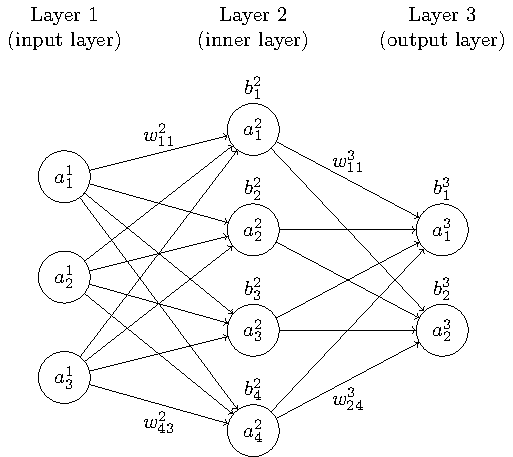
\includegraphics[scale=0.8]{smallNet.pdf}
			\caption{a neural network}
			\label{fig:smallNet}
		\end{figure}
		\begin{itemize}
			\item $a_j^\ell$ is the \emph{activation} of the $j\textsuperscript{th}$ neuron in the $\ell\textsuperscript{th}$ layer;
			\item $b_j^\ell$ is the \emph{bias} of the $j\textsuperscript{th}$ neuron in the $\ell\textsuperscript{th}$ layer (note that the first layer, called \emph{input layer}, has no biases);
			\item $w_{jk}^\ell$ is the \emph{weight} of the connection from the $k\textsuperscript{th}$ neuron in the $(\ell-1)\textsuperscript{th}$ layer to the $j\textsuperscript{th}$ neuron in the $\ell\textsuperscript{th}$ layer.
		\end{itemize}
		The activation of each neuron is the output of a sigmoid applied to a linear combination of the bias of that same neuron and the activations of the previous layer multiplied by their respective weights; for example
		$$
			a_3^2\defeq\sigma\!\left(w_{31}^2a_1^1+w_{32}^2a_2^1+w_{33}^2a_3^1+b_3^2\right),
		$$
		hence, in general,
		\begin{equation} \label{eq:activation}
			a_j^\ell\defeq\sigma\!\left(\sum_{k=1}^{m}w_{jk}^\ell\,a_k^{\ell-1}+b_j^\ell \right),
		\end{equation}
		where $m$ is the number of neurons in the $(\ell-1)\textsuperscript{th}$ layer. Therefore, by defining matrix $W^\ell$ and column vectors $a^\ell,b^\ell$ as 
		\begin{align*}
			\left(W^\ell\right)_{jk} &\defeq w_{jk}^\ell \\
			\left(a^\ell\right)_j    &\defeq a_j^\ell \\
			\left(b^\ell\right)_j	 &\defeq b_j^\ell,
		\end{align*}
		respectively, we can rewrite equation \ref{eq:activation} in the following matrix form:
		$$
			a^\ell=\sigma\!\left(W^\ell a^{\ell-1}+b^\ell\right).
		$$
	\end{definition}
	
	
	\chapter{Simulation of double-stack PDAs through neural networks} \chaptermark{Simulation} \label{chap:simulation}
	As an intermediate step in our construction, we will show how to simulate a double-stack PDA with a generic dynamical system.
	\begin{definition}
		Let $\mathcal{M}=(S,s_0,s_\h,\vartheta_0,\vartheta_1,\vartheta_2)$ be a double-stack PDA which computes $\varphi:\{0,1\}^* \to \{0,1\}^*$ and let $\mathcal{D}$ be a dynamical system with evolution function $g:\Q^n\to\Q^n$. We say $\mathcal{D}$ \emph{simulates} $\mathcal{M}$ if, given an encoding of the initial state $e[s_0]\in\Q^{n-2}$, an encoding of the halting state $e[s_\h]\in\Q^{n-2}$, and $\omega\in\{0,1\}^*$, $\varphi(\omega)$ is defined if and only if
		$$
			g^k(e[s_0],\delta[\omega],0)=(e[s_\h],\delta[\varphi(\omega)],\delta[\omega'])
		$$ 
		for some $k\in\mathbb{N}_{>0}$ and $\omega'\in\{0,1\}^*$.
	\end{definition}
	
	\begin{theorem} \label{theo:firstSimulation}
		\setcounter{theoremCounter}{\value{theorem}}
		Let $\mathcal{M}=(S,s_0,s_\h,\vartheta_0,\vartheta_1,\vartheta_2)$ be a double-stack PDA with $S=\{0,1,\dots,s\}$ computing $\varphi:\{0,1\}^* \to \{0,1\}^*$. Then, there exists a dynamical system with evolution function $g:\Q^{s+2}\to\Q^{s+2}$ simulating $\mathcal{M}$. 
	\end{theorem}
	
	\begin{proof}
		Define functions 
		$$
			\alpha_{ij}:\{0,1\}^4\to\{0,1\}
		$$ 
		for $i=0,1,\dots,s$, $j=1,2,\dots,s$ and 
		$$
			\beta_{ik}^\ell:\{0,1\}^4\to\{0,1\}
		$$
		for $k=1,2$, $\ell=1,2,3,4$ as follows:
		\begin{align*}
			\alpha_{ij}(a,b,d,e)=1 &\iff\vartheta_0(i,a,b,d,e)=j,\\ 
		\intertext{that is, iff, being $\mathcal{M}$ in state $i$ and having $a$ as top of stack one, $b$ as top of stack two, $d$ as the result of the nonemptiness test on stack one, and $e$ as the result of the nonemptiness test on stack two, $\mathcal{M}$ goes to state $j$;}
			\beta_{ik}^1(a,b,d,e)=1&\iff\vartheta_k(i,a,b,d,e)=(1,0,0),\\
		\intertext{that is, iff, being $\mathcal{M}$ in state $i$ and being $a,b,d,e$ the readings from the stacks, the content of stack $k$ does not change (i.e. the operation \noop{} occurs on stack $k$);}
			\beta_{ik}^2(a,b,d,e)=1&\iff\vartheta_k(i,a,b,d,e)=\left(\frac{1}{4},0,\frac{1}{4}\right),\\
		\intertext{that is, iff, being $\mathcal{M}$ in state $i$ and being $a,b,d,e$ the readings from the stacks, the operation \pushzero{} occurs on stack $k$;}
			\beta_{ik}^3(a,b,d,e)=1&\iff\vartheta_k(i,a,b,d,e)=\left(\frac{1}{4},0,\frac{3}{4}\right),\\
		\intertext{that is, iff, being $\mathcal{M}$ in state $i$ and being $a,b,d,e$ the readings from the stacks, the operation \pushone{} occurs on stack $k$;}
			\beta_{ik}^4(a,b,d,e)=1&\iff\vartheta_k(i,a,b,d,e)=(4,-2,-1),
		\end{align*}
		that is, iff, being $\mathcal{M}$ in state $i$ and being $a,b,d,e$ the readings from the stacks, the operation \pop{} occurs on stack $k$.
		
		Consider vectors of form $$(x_1,x_2,\dots,x_s,q_1,q_2)\in\Q^{s+2},$$ where $x_1,x_2,\dots,x_s\in\{0,1\}$ and $q_1,q_2\in Q$. The first $s$ components are used to encode the state $\mathcal{M}$ is in, with $i\in S\setminus\{0\}$ corresponding to the $i\textsuperscript{th}$ canonical vector $$e_i\defeq(0,\dots,0,1,0,\dots,0)\in\Q^s,$$ where the 1 is in the $i\textsuperscript{th}$ position, and $0\in S$ corresponding to $$e_0\defeq(0,0,\dots,0)\in\Q^s;$$ $q_1$ and $q_2$, on the other hand, encode the contents of stack one and two, respectively.
		
		Let $g:\Q^{s+2}\to\Q^{s+2}$ be defined by 
		\begin{equation} \label{eq:g}
			g(x_1,x_2,\dots,x_s,q_1,q_2)\defeq(x_1^+,x_2^+,\dots,x_s^+,q_1^+,q_2^+),
		\end{equation} 
		where, denoting $x_0\defeq1-\sum_{j=1}^{s}x_j$,
		\begin{equation} \label{eq:state}
			x_j^+\defeq\sum_{i=0}^{s}\alpha_{ij}(\zeta[q_1],\zeta[q_2],\tau[q_1],\tau[q_2])x_i
		\end{equation}
		for $j=1,2,\dots,s$ and
		\begin{align} \label{eq:stacks}
			\begin{split}
				q_k^+\defeq &\left(\sum_{i=0}^{s}\beta_{ik}^1(\zeta[q_1],\zeta[q_2],\tau[q_1],\tau[q_2])x_i\right)q_k\:+ \\
							&\left(\sum_{i=0}^{s}\beta_{ik}^2(\zeta[q_1],\zeta[q_2],\tau[q_1],\tau[q_2])x_i\right)
								\left(\frac{1}{4}q_k+\frac{1}{4}\right) + \\
							&\left(\sum_{i=0}^{s}\beta_{ik}^3(\zeta[q_1],\zeta[q_2],\tau[q_1],\tau[q_2])x_i\right)
								\left(\frac{1}{4}q_k+\frac{3}{4}\right) + \\
							&\left(\sum_{i=0}^{s}\beta_{ik}^4(\zeta[q_1],\zeta[q_2],\tau[q_1],\tau[q_2])x_i\right)
								\left(4q_k-2\zeta[q_k]-1\right)
			\end{split}
		\end{align}
		for $k=1,2$. 
		
		Let $f$ be the transition function of $\mathcal{M}$ and let $\pi:S\times Q\times Q\to\Q^{s+2}$ be defined by 
		\begin{equation}
			\pi[i,q_1,q_2] \defeq (e_i,q_1,q_2). \label{eq:pi}
		\end{equation} 
		It follows immediately from equations \ref{eq:state} and \ref{eq:stacks} that, for any $(i,q_1,q_2)\in S\times Q\times Q$,
		$$
			g(\pi[i,q_1,q_2])=\pi[f(i,q_1,q_2)],
		$$
		which, applied repeatedly, becomes 
		\begin{equation} \label{eq:equivalence}
			g^k(\pi[i,q_1,q_2])=\pi[f^k(i,q_1,q_2)]
		\end{equation}
		for all $k\in\mathbb{N}_{>0}$. 
		
		Assume, without loss of generality, that $s_0=0$ and $s_\h=1$, and let $\omega\in\{0,1\}^*$. Then, $\varphi(\omega)$ is defined if and only if
		\begin{align*}
			g^\ell(e_0,\delta[\omega],0) &= g^\ell(\pi[0,\delta[\omega],0]) \tag{by equation \ref{eq:pi}} \\
										 &= \pi[f^\ell(0,\delta[\omega],0)] \tag{by equation \ref{eq:equivalence}} \\
										 &= \pi[1,\delta[\varphi(\omega)],\delta[\omega']] \tag{by definition \ref{def:computed}} \\
										 &= (e_1,\delta[\varphi(\omega)],\delta[\omega']) \tag{by equation \ref{eq:pi}}
		\end{align*}
		for some $\ell\in\mathbb{N}_{>0}$ and $\omega'\in\{0,1\}^*$, i.e. $g$ is the evolution function of a dynamical system which simulates $\mathcal{M}$.
	\end{proof}
	
	Now that we have seen how to simulate a double-stack PDA with a generic dynamical system with evolution function $g:\Q^{s+2}\to\Q^{s+2}$, we will show how to implement $g$ with a neural network. We first need the following technical lemma:
	
	\begin{lemma} \label{theo:lemma}
		Let $\alpha:\{0,1\}^4\to\{0,1\}$, $a,b,d,e,x\in\{0,1\}$, and $q\in[0,1)$. Then, there exist vectors $$v_1,v_2,\dots,v_{16}\in\mathbb{Z}^6$$ and scalars $$c_1,c_2,\dots,c_{16}\in\{0,1\}$$ such that
		\begin{equation}
			\alpha(a,b,d,e)x=\sum_{m=1}^{16}c_m\sigma(v_m\cdot\eta) \label{eq:lemmaState}
		\end{equation}
		and
		$$
			\alpha(a,b,d,e)xq=\sigma\!\left(q-1+\sum_{m=1}^{16}c_m\sigma(v_m\cdot\eta)\right),
		$$
		where $\eta\defeq(1,a,b,d,e,x)$ and $\cdot$ is the dot product in $\mathbb{Z}^6$.
	\end{lemma}
	
	\begin{proof}
		The fact that $\alpha$ goes from $\{0,1\}^4$ to $\{0,1\}$ allows us to write it as a polynomial (see table \ref{tab:polynomial}):
		\begin{table}[t]
	\centering
	\begin{tabular}{|c c c c c|}
		\hline 
		$a$ & $b$ & $d$ & $e$ & Term in the polynomial \\
		\hline
		0 & 0 & 0 & 0 & $c_1$        \\
		0 & 0 & 0 & 1 & $c_2e$       \\
		0 & 0 & 1 & 0 & $c_3d$       \\
		0 & 0 & 1 & 1 & $c_4de$      \\
		0 & 1 & 0 & 0 & $c_5b$       \\
		0 & 1 & 0 & 1 & $c_6be$      \\
		0 & 1 & 1 & 0 & $c_7bd$      \\
		0 & 1 & 1 & 1 & $c_8bde$     \\
		1 & 0 & 0 & 0 & $c_9a$       \\
		1 & 0 & 0 & 1 & $c_{10}ae$   \\
		1 & 0 & 1 & 0 & $c_{11}ad$   \\
		1 & 0 & 1 & 1 & $c_{12}ade$  \\
		1 & 1 & 0 & 0 & $c_{13}ab$   \\
		1 & 1 & 0 & 1 & $c_{14}abe$  \\
		1 & 1 & 1 & 0 & $c_{15}abd$  \\
		1 & 1 & 1 & 1 & $c_{16}abde$ \\
		\hline
	\end{tabular}
	\caption{$\alpha:\{0,1\}^4\to\{0,1\}$ as a polynomial}
	\label{tab:polynomial}
\end{table}
		\begin{align*}
			\alpha(a,b,d,e)=\;&c_1+c_2e+c_3d+c_4de\:+\\
							  &c_5b+c_6be+c_7bd+c_8bde\:+\\
							  &c_9a+c_{10}ae+c_{11}ad+c_{12}ade\:+\\
							  &c_{13}ab+c_{14}abe+c_{15}abd+c_{16}abde
		\end{align*}
		for some $c_1,c_2,\dots,c_{16}\in\{0,1\}$, and thus
		\begin{align} \label{eq:polynomial}
			\begin{split}
				\alpha(a,b,d,e)x=\;&c_1x+c_2ex+c_3dx+c_4dex\:+\\
								   &c_5bx+c_6bex+c_7bdx+c_8bdex\:+\\
								   &c_9ax+c_{10}aex+c_{11}adx+c_{12}adex\:+\\
								   &c_{13}abx+c_{14}abex+c_{15}abdx+c_{16}abdex.
			\end{split}
		\end{align}
		
		Note that, for any $a_1,a_2,\dots,a_k\in\{0,1\}$ with $k\in\mathbb{N}_{>0}$ and $p\in[0,1]$, one has
		\begin{equation} \label{eq:towardsLemmaState}
			a_1a_2\dots a_kp=\sigma(a_1+a_2+\dots+a_k-k+p).
		\end{equation}
		In fact, if there exists $ i\in\{1,2,\dots,k\}$ such that $a_i=0$, then $a_1+a_2+\dots+a_k\leq k-1$, and thus $a_1+a_2+\dots+a_k-k+p\leq k-1-k+p=p-1\in[-1,0]$, hence $\sigma(a_1+a_2+\dots+a_k-k+p)=0=a_1a_2\dots a_kp$; on the other hand, if $a_i=1$ for all $i\in\{1,2,\dots,k\}$, then $a_1+a_2+\dots+a_k=k$, and thus $a_1+a_2+\dots+a_k-k+p=k-k+p=p\in[0,1]$, hence $\sigma(a_1+a_2+\dots+a_k-k+p)=p=a_1a_2\dots a_kp$.
		
		Therefore, we can rewrite the terms of equation \ref{eq:polynomial} as (consider $p=1$)
		\begingroup
		\allowdisplaybreaks
		\begin{align*} 
			c_1x    	&= c_1\sigma(x) \\
						&= c_1\sigma((0,0,0,0,0,1)\cdot(1,a,b,d,e,x)) \\
			c_2ex    	&= c_2\sigma(e+x-1) \\
						&= c_2\sigma((-1,0,0,0,1,1)\cdot(1,a,b,d,e,x)) \\
			c_3dx    	&= c_3\sigma(d+x-1) \\
						&= c_3\sigma((-1,0,0,1,0,1)\cdot(1,a,b,d,e,x)) \\
			c_4dex    	&= c_4\sigma(d+e+x-2) \\
						&= c_4\sigma((-2,0,0,1,1,1)\cdot(1,a,b,d,e,x)) \\
			c_5bx       &= c_5\sigma(b+x-1) \\
						&= c_5\sigma((-1,0,1,0,0,1)\cdot(1,a,b,d,e,x)) \\
			c_6bex      &= c_6\sigma(b+e+x-2) \\
						&= c_6\sigma((-2,0,1,0,1,1)\cdot(1,a,b,d,e,x)) \\
			c_7bdx      &= c_7\sigma(b+d+x-2) \\
						&= c_7\sigma((-2,0,1,1,0,1)\cdot(1,a,b,d,e,x)) \\
			c_8bdex     &= c_8\sigma(b+d+e+x-3) \\
						&= c_8\sigma((-3,0,1,1,1,1)\cdot(1,a,b,d,e,x)) \\
			c_9ax    	&= c_9\sigma(a+x-1) \\
						&= c_9\sigma((-1,1,0,0,0,1)\cdot(1,a,b,d,e,x)) \\
			c_{10}aex   &= c_{10}\sigma(a+e+x-2) \\
						&= c_{10}\sigma((-2,1,0,0,1,1)\cdot(1,a,b,d,e,x)) \\
			c_{11}adx 	&= c_{11}\sigma(a+d+x-2) \\
						&= c_{11}\sigma((-2,1,0,1,0,1)\cdot(1,a,b,d,e,x)) \\
			c_{12}adex 	&= c_{12}\sigma(a+d+e+x-3) \\
						&= c_{12}\sigma((-3,1,0,1,1,1)\cdot(1,a,b,d,e,x)) \\
			c_{13}abx 	&= c_{13}\sigma(a+b+x-2) \\
						&= c_{13}\sigma((-2,1,1,0,0,1)\cdot(1,a,b,d,e,x)) \\
			c_{14}abex  &= c_{14}\sigma(a+b+e+x-3) \\
						&= c_{14}\sigma((-3,1,1,0,1,1)\cdot(1,a,b,d,e,x)) \\
			c_{15}abdx  &= c_{15}\sigma(a+b+d+x-3) \\
						&= c_{15}\sigma((-3,1,1,1,0,1)\cdot(1,a,b,d,e,x)) \\
			c_{16}abdex &= c_{16}\sigma(a+b+d+e+x-4) \\
						&= c_{16}\sigma((-4,1,1,1,1,1)\cdot(1,a,b,d,e,x)),
		\end{align*}
		\endgroup
		hence 
		$$ 
			\alpha(a,b,d,e)x=\sum_{m=1}^{16}c_m\sigma(v_m\cdot\eta)
		$$
		for some $c_1,c_2,\dots,c_{16}\in\{0,1\}$ and $v_1,v_2,\dots,v_{16}\in\mathbb{Z}^6$.
		
		Note also that, for any $c\in\{0,1\}$ and $r\in[0,1)$, it holds that 
		\begin{equation} \label{eq:towardsLemmaStacks}
			cr=\sigma(r-1+c).
		\end{equation}
		In fact, if $c=0$, then $r-1+c=r-1\in[-1,0)$, hence $\sigma(r-1+c)=0=cr$; on the other hand, if $c=1$, then $r-1+c=r\in[0,1)$, hence $\sigma(r-1+c)=r=cr$.
		
		Therefore, by equations \ref{eq:lemmaState} and \ref{eq:towardsLemmaStacks},
		$$
			\alpha(a,b,d,e)xq=\sigma\!\left(q-1+\sum_{m=1}^{16}c_m\sigma(v_m\cdot\eta)\right)
		$$
		for some $c_1,c_2,\dots,c_{16}\in\{0,1\}$ and $v_1,v_2,\dots,v_{16}\in\mathbb{Z}^6$.
	\end{proof}
	
	\begin{remark} \label{theo:9not16}
		Note that, if the $\alpha$ from lemma \ref{theo:lemma} stands for the $\alpha_{ij}$s or the $\beta_{ik}^\ell$s from theorem \ref{theo:firstSimulation}, then $a=\zeta[q_1],b=\zeta[q_2],d=\tau[q_1],e=\tau[q_2]$, and since, as we already pointed out in definition \ref{def:topAndNonempty}, it can never happen that $(\zeta[q_1]=1\land\tau[q_1]=0)\lor(\zeta[q_2]=1\land\tau[q_2]=0)$, i.e. $(a=1\land d=0)\lor(b=1\land e=0)$, we just need nine out of the sixteen $c_1,c_2,\dots,c_{16}$ to write $\alpha$ as a polynomial (see table \ref{tab:reducedPolynomial}):
		\begin{table}[t]
	\centering
	\begin{tabular}{|c c c c c c|}
		\hline 
		$a$ & $b$ & $d$ & $e$ & Term in the polynomial & $v_m$ \\
		\hline
		0 & 0 & 0 & 0 & $c_1$     & $(0,0,0,0,0,1)$ \\
		0 & 0 & 0 & 1 & $c_2e$    & $(-1,0,0,0,1,1)$ \\
		0 & 0 & 1 & 0 & $c_3d$    & $(-1,0,0,1,0,1)$ \\
		0 & 0 & 1 & 1 & $c_4de$   & $(-2,0,0,1,1,1)$ \\
		0 & 1 & 0 & 0 & 0         & \\
		0 & 1 & 0 & 1 & $c_5be$   & $(-2,0,1,0,1,1)$ \\
		0 & 1 & 1 & 0 & 0         & \\
		0 & 1 & 1 & 1 & $c_6bde$  & $(-3,0,1,1,1,1)$\\
		1 & 0 & 0 & 0 & 0         & \\
		1 & 0 & 0 & 1 & 0         & \\
		1 & 0 & 1 & 0 & $c_7ad$   & $(-2,1,0,1,0,1)$\\
		1 & 0 & 1 & 1 & $c_8ade$  & $(-3,1,0,1,1,1)$\\
		1 & 1 & 0 & 0 & 0         & \\
		1 & 1 & 0 & 1 & 0         & \\
		1 & 1 & 1 & 0 & 0         & \\
		1 & 1 & 1 & 1 & $c_9abde$ & $(-4,1,1,1,1,1)$ \\
		\hline
	\end{tabular}
	\caption{$\alpha_{ij}$s and $\beta_{ik}^\ell$s as polynomials}
	\label{tab:reducedPolynomial}
\end{table}
		\begin{align*}
			\alpha(a,b,d,e)=\;&c_1+c_2e+c_3d+c_4de+c_5be\:+ \\
							  &c_6bde+c_7ad+c_8ade+c_9abde,
		\end{align*}
		hence
		\begin{equation}
			\alpha(a,b,d,e)x=\sum_{m=1}^{9}c_m\sigma(v_m\cdot\eta) \label{eq:reducedLemmaState}
		\end{equation}
		and
		$$
			\alpha(a,b,d,e)xq=\sigma\!\left(q-1+\sum_{m=1}^{9}c_m\sigma(v_m\cdot\eta)\right).
		$$
	\end{remark}
	
	\setcounter{theorem}{\thetheoremCounter}
	\begin{corollary} \label{theo:secondSimulation}
		Let $\mathcal{M}=(S,s_0,s_\h,\vartheta_0,\vartheta_1,\vartheta_2)$ be a double-stack PDA with $S=\{0,1,\dots,s\}$ computing $\varphi:\{0,1\}^*\to\{0,1\}^*$. Then, there exists a neural network with evolution function $g:\Q^{s+2}\to\Q^{s+2}$ simulating $\mathcal{M}$.
	\end{corollary}
	
	\begin{proof}
		Apply equation \ref{eq:reducedLemmaState} to equation \ref{eq:state}, where $\alpha=\alpha_{ij}$ and $x=x_i$. Furthermore, write $\sigma(4q_k-2)$ whenever $\zeta[q_k]$ appears (see equation \ref{eq:top}) and $\sigma(4q_k)$ whenever $\tau[q_k]$ appears (see equation \ref{eq:nonempty}). Finally, note that $x_j^+=\sigma\!\left(x_j^+\right)$, since $x_j^+\in\{0,1\}$. This way, equation \ref{eq:state} becomes
		\begin{equation} \label{eq:netState}
			x_j^+=\sigma\!\left(\sum_{i=0}^{s}\sum_{m=1}^{9}c_{ijm}\sigma_{im}\right),
		\end{equation}
		where
		\begin{equation} \label{eq:sigma_im}
			\sigma_{im}\defeq\sigma(v_m\cdot(1,\sigma(4q_1-2),\sigma(4q_2-2),\sigma(4q_1),\sigma(4q_2),x_i))
		\end{equation}
		(the $v_m$s are shown in table \ref{tab:reducedPolynomial}).
		
		On the other hand, apply equation \ref{eq:towardsLemmaStacks} to equation \ref{eq:stacks}, where $c=\sum_{i=0}^{s}\beta_{ik}^\ell(\dots)x_i$ and $r=q_k$, $r=\frac{1}{4}q_k+\frac{1}{4}$, $r=\frac{1}{4}q_k+\frac{3}{4}$, or $r=4q_k-2\zeta[q_k]-1$. Again, write $\sigma(4q_k-2)$ whenever $\zeta[q_k]$ appears and $\sigma(4q_k)$ whenever $\tau[q_k]$ appears. Finally, note that $q_k^+=\sigma\!\left(q_k^+\right)$, since $q_k\in[0,1)$. This way, equation \ref{eq:stacks} becomes
		\begin{align*}  
			q_k^+=\sigma\Bigg(&\sigma\Bigg(q_k-1+\sum_{i=0}^{s}\beta_{ik}^1(
								  \sigma(4q_1-2),\sigma(4q_2-2),\sigma(4q_1),\sigma(4q_2))x_i\Bigg)+ \\
							  &\sigma\Bigg(\frac{1}{4}q_k+\frac{1}{4}-1+\sum_{i=0}^{s}\beta_{ik}^2(
								  \sigma(4q_1-2),\sigma(4q_2-2),\sigma(4q_1),\sigma(4q_2))x_i\Bigg)+ \\
							  &\sigma\Bigg(\frac{1}{4}q_k+\frac{3}{4}-1+\sum_{i=0}^{s}\beta_{ik}^3(
								  \sigma(4q_1-2),\sigma(4q_2-2),\sigma(4q_1),\sigma(4q_2))x_i\Bigg)+ \\
							  &\sigma\Bigg(4q_k-2\sigma(4q_k-2)-1-1\:+\sum_{i=0}^{s}\beta_{ik}^4(
								  \sigma(4q_1-2),\sigma(4q_2-2),\sigma(4q_1),\sigma(4q_2))x_i\Bigg)\Bigg).
		\end{align*}
		Now, if we apply equation \ref{eq:reducedLemmaState} with $x=x_i$ and $\alpha=\beta_{ik}^1$, $\alpha=\beta_{ik}^2$, $\alpha=\beta_{ik}^3$, or $\alpha=\beta_{ik}^4$, we get
		\begin{equation} \label{eq:netStacks}
			q_k^+=\sigma\!\left(q_{k1}^++q_{k2}^++q_{k3}^++q_{k4}^+\right),
		\end{equation}
		where 
		\begin{align} \label{eq:q_kl+}
			\begin{split}
				q_{k1}^+\defeq\sigma\!&\left(q_k-1+\sum_{i=0}^{s}\sum_{m=1}^{9}c_{ikm}^1\sigma_{im}\right) \\
				q_{k2}^+\defeq\sigma\!&\left(\frac{1}{4}q_k-\frac{3}{4}+\sum_{i=0}^{s}\sum_{m=1}^{9}c_{ikm}^2\sigma_{im}\right) \\
				q_{k3}^+\defeq\sigma\!&\left(\frac{1}{4}q_k-\frac{1}{4}+\sum_{i=0}^{s}\sum_{m=1}^{9}c_{ikm}^3\sigma_{im}\right) \\
				q_{k4}^+\defeq\sigma\!&\left(4q_k-2\sigma(4q_k-2)-2+\sum_{i=0}^{s}\sum_{m=1}^{9}c_{ikm}^4\sigma_{im}\right).
			\end{split}
		\end{align}
		
		Write $g$ as a composition $$g=g_4\circ g_3\circ g_2\circ g_1$$ of four functions of form $\sigma(Wx+b)$: 
		\begin{align*}
			g_1&:\Q^{s+2}\to\Q^{s+7} \\
			g_2&:\Q^{s+7}\to\Q^{9s+13} \\
			g_3&:\Q^{9s+13}\to\Q^{s+8} \\
			g_4&:\Q^{s+8}\to \Q^{s+2}.
		\end{align*}
		Each of those functions computes a piece of equations \ref{eq:netState} and \ref{eq:netStacks} and corresponds to a layer of the neural network $\mathcal{N}$ shown in figure \ref{fig:net}:
		\begin{figure}[t]
			\centering
			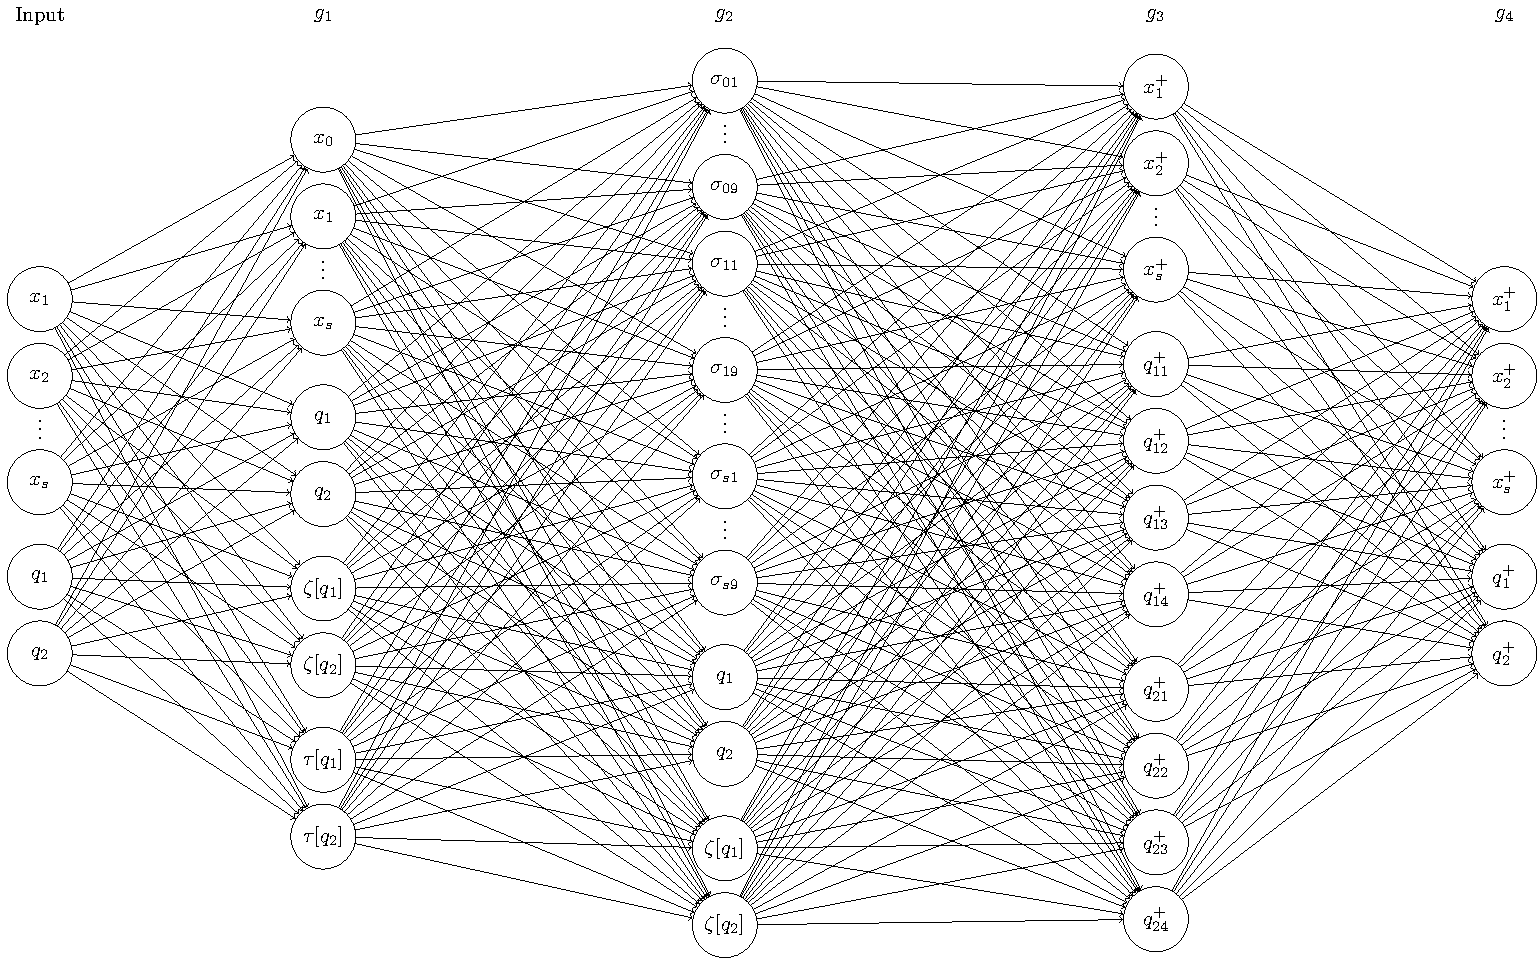
\includegraphics[width=\textwidth]{netImage.pdf}
			\caption{a recurrent neural network simulating a generic double-stack PDA}
			\label{fig:net}
		\end{figure}
		\begin{itemize}
			\item $g_1$: 
			\begin{itemize}
				\item Input: the same as $g$ (see equation \ref{eq:g}), i.e. $x_1,x_2,\dots,x_s,q_1,q_2$;
				\item Computes: $x_0=1-\sum_{j=1}^{s}x_j$ (as defined in theorem \ref{theo:firstSimulation}), $\zeta[q_k]=\sigma(4q_k-2)$, and $\tau[q_k]=\sigma(4q_k)$, for $k=1,2$;
				\item Output: $x_0,x_1,\dots,x_s,q_1,q_2,\zeta[q_k],\tau[q_k]$, for $k=1,2$;
			\end{itemize}
			
			\item $g_2$:
			\begin{itemize}
				\item Input: $x_0,x_1,\dots,x_s,q_1,q_2,\zeta[q_k],\tau[q_k]$, for $k=1,2$;
				\item Computes: the $\sigma_{im}$s of equation \ref{eq:sigma_im}, for $i=0,1\dots,s$ and $m=1,2,\dots,9$;
				\item Output: $\sigma_{im},q_k,\zeta[q_k]$, for $i=0,1\dots,s$, $m=1,2,\dots,9$, and $k=1,2$;
			\end{itemize}
			\item $g_3$:
			\begin{itemize}
				\item Input: $\sigma_{im},q_k,\zeta[q_k]$, for $i=0,1\dots,s$, $m=1,2,\dots,9$, and $k=1,2$;
				\item Computes: the $x_j^+$s of equation \ref{eq:netState} and the $q_{k\ell}^+$s of equations \ref{eq:q_kl+}, for $j=1,2,\dots,s$, $k=1,2$, and $\ell=1,2,3,4$;
				\item Output: $x_j^+,q_{k\ell}^+$, for $j=1,2,\dots,s$, $k=1,2$, and $\ell=1,2,3,4$;
			\end{itemize}
			\item $g_4$:
			\begin{itemize}
				\item Input: $x_j^+,q_{k\ell}^+$, for $j=1,2,\dots,s$, $k=1,2$, and $\ell=1,2,3,4$;
				\item Computes: the $q_k^+$s of equation \ref{eq:netStacks}, for $k=1,2$;
				\item Output: $x_j^+,q_k^+$, for $j=1,2,\dots,s$ and $k=1,2$.
			\end{itemize}
		\end{itemize}
		The output of $g_4$ becomes then the input of $g_1$ for the next iteration of $g$; $\mathcal{N}$ is therefore referred to as a \emph{recurrent} neural network. The weight matrices and bias vectors of $\mathcal{N}$ are shown in tables \ref{tab:W1b1}, \ref{tab:W2b2}, \ref{tab:W3b3}, and \ref{tab:W4b4}.
		\begin{table}[p]
	\centering
	\begin{tabular}{|c| c c c c c c |c|}
		\hline 
		$W^1$ & $x_1$ & $x_2$ & $\cdots$ & $x_s$ & $q_1$ & $q_2$ & $b^1$ \\
		\hline
		$x_0$ & $-1$ & $-1$ & $\cdots$ & $-1$ & 0 & 0 & 1 \\
		$x_1$ & 1 & 0 & $\cdots$ & 0 & 0 & 0 & 0 \\
		$\vdots$ & $\vdots$ & $\vdots$ & $\ddots$ & $\vdots$ & $\vdots$ & $\vdots$ & $\vdots$ \\
		$x_s$ & 0 & 0 & $\cdots$ & 1 & 0 & 0 & 0 \\
		$q_1$ & 0 & 0 & $\cdots$ & 0 & 1 & 0 & 0 \\
		$q_2$ & 0 & 0 & $\cdots$ & 0 & 0 & 1 & 0 \\
		$\zeta[q_1]$ & 0 & 0 & $\cdots$ & 0 & 4 & 0 & $-2$ \\
		$\zeta[q_2]$ & 0 & 0 & $\cdots$ & 0 & 0 & 4 & $-2$ \\
		$\tau[q_1]$ & 0 & 0 & $\cdots$ & 0 & 4 & 0 & 0 \\
		$\tau[q_2]$ & 0 & 0 & $\cdots$ & 0 & 0 & 4 & 0 \\
		\hline
	\end{tabular}
	\caption{weights from the input layer to the $g_1$ layer and biases of the $g_1$ layer}
	\label{tab:W1b1}
\end{table}
		\begin{table}[p]
	\centering
	\begin{tabular}{|c| c c c c c c c c c c |c|}
		\hline 
		$W^2$ & $x_0$ & $x_1$ & $\cdots$ & $x_s$ & $q_1$ & $q_2$ & $\zeta[q_1]$ & $\zeta[q_2]$ & $\tau[q_1]$ & $\tau[q_2]$ & $b^2$ \\
		\hline
		$\sigma_{01}$ & 1 & 0 & $\cdots$ & 0 & 0 & 0 & 0 & 0 & 0 & 0 & 0 \\
		$\vdots$ & $\vdots$ & $\vdots$ & $\ddots$ & $\vdots$ & $\vdots$ & $\vdots$ & $\vdots$ & $\vdots$ & $\vdots$ & $\vdots$ & $\vdots$ \\
		$\sigma_{09}$ & 1 & 0 & $\cdots$ & 0 & 0 & 0 & 1 & 1 & 1 & 1 & $-4$ \\
		$\sigma_{11}$ & 0 & 1 & $\cdots$ & 0 & 0 & 0 & 0 & 0 & 0 & 0 & 0 \\
		$\vdots$ & $\vdots$ & $\vdots$ & $\ddots$ & $\vdots$ & $\vdots$ & $\vdots$ & $\vdots$ & $\vdots$ & $\vdots$ & $\vdots$ & $\vdots$ \\
		$\sigma_{19}$ & 0 & 1 & $\cdots$ & 0 & 0 & 0 & 1 & 1 & 1 & 1 & $-4$ \\
		$\vdots$ & $\vdots$ & $\vdots$ & $\ddots$ & $\vdots$ & $\vdots$ & $\vdots$ & $\vdots$ & $\vdots$ & $\vdots$ & $\vdots$ & $\vdots$ \\
		$\sigma_{s1}$ & 0 & 0 & $\cdots$ & 1 & 0 & 0 & 0 & 0 & 0 & 0 & 0 \\
		$\vdots$ & $\vdots$ & $\vdots$ & $\ddots$ & $\vdots$ & $\vdots$ & $\vdots$ & $\vdots$ & $\vdots$ & $\vdots$ & $\vdots$ & $\vdots$ \\
		$\sigma_{s9}$ & 0 & 0 & $\cdots$ & 1 & 0 & 0 & 1 & 1 & 1 & 1 & $-4$ \\
		$q_1$ & 0 & 0 & $\cdots$ & 0 & 1 & 0 & 0 & 0 & 0 & 0 & 0 \\
		$q_2$ & 0 & 0 & $\cdots$ & 0 & 0 & 1 & 0 & 0 & 0 & 0 & 0 \\
		$\zeta[q_1]$ & 0 & 0 & $\cdots$ & 0 & 0 & 0 & 1 & 0 & 0 & 0 & 0 \\
		$\zeta[q_2]$ & 0 & 0 & $\cdots$ & 0 & 0 & 0 & 0 & 1 & 0 & 0 & 0 \\
		\hline
	\end{tabular}
	\caption{weights from the $g_1$ layer to the $g_2$ layer and biases of the $g_2$ layer}
	\label{tab:W2b2}
\end{table}
		\begin{table}[p]
	\centering
	\begin{tabular}{|c| c c c c c c c c c c c c c c |c|}
		\hline 
		$W^3$ & $\sigma_{01}$ & $\cdots$ & $\sigma_{09}$ & $\sigma_{11}$ & $\cdots$ & $\sigma_{19}$ & $\cdots$ & $\sigma_{s1}$ & $\cdots$ & $\sigma_{s9}$ & $q_1$ & $q_2$ & $\zeta[q_1]$ & $\zeta[q_2]$ & $b^3$ \\
		\hline
		$x_1^+$ & $c_{011}$ & $\cdots$ & $c_{019}$ & $c_{111}$ & $\cdots$ & $c_{119}$ & $\cdots$ & $c_{s11}$ & $\cdots$ & $c_{s19}$ & 0 & 0 & 0 & 0 & 0 \\
		$x_2^+$ & $c_{021}$ & $\cdots$ & $c_{029}$ & $c_{121}$ & $\cdots$ & $c_{129}$ & $\cdots$ & $c_{s21}$ & $\cdots$ & $c_{s29}$ & 0 & 0 & 0 & 0 & 0 \\
		$\vdots$ & $\vdots$ & $\ddots$ & $\vdots$ & $\vdots$ & $\ddots$ & $\vdots$ & $\ddots$ & $\vdots$ & $\ddots$ & $\vdots$ & $\vdots$ & $\vdots$ & $\vdots$ & $\vdots$ & $\vdots$ \\
		$x_s^+$ & $c_{0s1}$ & $\cdots$ & $c_{0s9}$ & $c_{1s1}$ & $\cdots$ & $c_{1s9}$ & $\cdots$ & $c_{ss1}$ & $\cdots$ & $c_{ss9}$ & 0 & 0 & 0 & 0 & 0 \\
				
		$q_{11}^+$ & $c_{011}^1$ & $\cdots$ & $c_{019}^1$ & $c_{111}^1$ & $\cdots$ & $c_{119}^1$ & $\cdots$ & $c_{s11}^1$ & $\cdots$ & $c_{s19}^1$ & 1 & 0 & 0 & 0 & $-1$ \\
		$q_{12}^+$ & $c_{011}^2$ & $\cdots$ & $c_{019}^2$ & $c_{111}^2$ & $\cdots$ & $c_{119}^2$ & $\cdots$ & $c_{s11}^2$ & $\cdots$ & $c_{s19}^2$ & $\frac{1}{4}$ & 0 & 0 & 0 & $-\frac{3}{4}$ \\
		$q_{13}^+$ & $c_{011}^3$ & $\cdots$ & $c_{019}^3$ & $c_{111}^3$ & $\cdots$ & $c_{119}^3$ & $\cdots$ & $c_{s11}^3$ & $\cdots$ & $c_{s19}^3$ & $\frac{1}{4}$ & 0 & 0 & 0 & $-\frac{1}{4}$ \\
		$q_{14}^+$ & $c_{011}^4$ & $\cdots$ & $c_{019}^4$ & $c_{111}^4$ & $\cdots$ & $c_{119}^4$ & $\cdots$ & $c_{s11}^4$ & $\cdots$ & $c_{s19}^4$ & 4 & 0 & $-2$ & 0 & $-2$ \\
				
		$q_{21}^+$ & $c_{021}^1$ & $\cdots$ & $c_{029}^1$ & $c_{121}^1$ & $\cdots$ & $c_{129}^1$ & $\cdots$ & $c_{s21}^1$ & $\cdots$ & $c_{s29}^1$ & 0 & 1 & 0 & 0 & $-1$ \\
		$q_{22}^+$ & $c_{021}^2$ & $\cdots$ & $c_{029}^2$ & $c_{121}^2$ & $\cdots$ & $c_{129}^2$ & $\cdots$ & $c_{s21}^2$ & $\cdots$ & $c_{s29}^2$ & 0 & $\frac{1}{4}$ & 0 & 0 & $-\frac{3}{4}$ \\
		$q_{23}^+$ & $c_{021}^3$ & $\cdots$ & $c_{029}^3$ & $c_{121}^3$ & $\cdots$ & $c_{129}^3$ & $\cdots$ & $c_{s21}^3$ & $\cdots$ & $c_{s29}^3$ & 0 & $\frac{1}{4}$ & 0 & 0 & $-\frac{1}{4}$ \\
		$q_{24}^+$ & $c_{021}^4$ & $\cdots$ & $c_{029}^4$ & $c_{121}^4$ & $\cdots$ & $c_{129}^4$ & $\cdots$ & $c_{s21}^4$ & $\cdots$ & $c_{s29}^4$ & 0 & 4 & 0 & $-2$ & $-2$ \\
		\hline
	\end{tabular}
	\caption{weights from the $g_2$ layer to the $g_3$ layer and biases of the $g_3$ layer}
	\label{tab:W3b3}
\end{table}
		\begin{table}[p]
	\centering
	\begin{tabular}{|c| c c c c c c c c c c c c |c|}
		\hline 
		$W^4$ & $x_1^+$ & $x_2^+$ & $\cdots$ & $x_s^+$ & $q_{11}^+$ & $q_{12}^+$ & $q_{13}^+$ & $q_{14}^+$ & $q_{21}^+$ & $q_{22}^+$ & $q_{23}^+$ & $q_{24}^+$ & $b^4$ \\
		\hline
		$x_1^+$ & 1 & 0 & $\cdots$ & 0 & 0 & 0 & 0 & 0 & 0 & 0 & 0 & 0 & 0 \\
		$x_2^+$ & 0 & 1 & $\cdots$ & 0 & 0 & 0 & 0 & 0 & 0 & 0 & 0 & 0 & 0 \\
		$\vdots$ & $\vdots$ & $\vdots$ & $\ddots$ & $\vdots$ & $\vdots$ & $\vdots$ & $\vdots$ & $\vdots$ & $\vdots$ & $\vdots$ & $\vdots$ & $\vdots$ & $\vdots$ \\
		$x_s^+$ & 0 & 0 & $\cdots$ & 1 & 0 & 0 & 0 & 0 & 0 & 0 & 0 & 0 & 0 \\
		$q_1^+$ & 0 & 0 & $\cdots$ & 0 & 1 & 1 & 1 & 1 & 0 & 0 & 0 & 0 & 0 \\
		$q_2^+$ & 0 & 0 & $\cdots$ & 0 & 0 & 0 & 0 & 0 & 1 & 1 & 1 & 1 & 0 \\
		\hline
	\end{tabular}
	\caption{weights from the $g_3$ layer to the $g_4$ layer and biases of the $g_4$ layer}
	\label{tab:W4b4}
\end{table}
		
		We have already proved in theorem \ref{theo:firstSimulation} that $g$ is the evolution function of a dynamical system $\mathcal{D}$ which simulates $\mathcal{M}$, assuming, without loss of generality, that $s_0=0$ and $s_\h=1$ (encoded in $\mathcal{D}$ by $e_0$ and $e_1$, respectively). On the other hand, we have just built a neural network $\mathcal{N}$ implementing $g$. Thus, given $\omega\in\{0,1\}^*$, $\varphi(\omega)$ is defined if and only if an input layer $x_1=x_2=\dots=x_s=0$ (i.e. $e_0$), $q_1=\delta[\omega],q_2=0$ eventually causes $\mathcal{N}$ to output in the $g_4$ layer $x_1^+=1,x_2^+=x_3^+=\dots=x_s^+=0$ (i.e. $e_1$), $q_1^+=\delta[\varphi(\omega)]$ (and some $q_2^+\in Q$).
	\end{proof}
	
	\chapter{An example}
	\section{Formal construction} \label{sec:mathex}
	We are now going to apply the formal construction of chapter \ref{chap:simulation} to a specific example to get a more compact and concrete overview of how it actually operates. In the following discussion, mostly based on \cite{slides}, we will not precisely follow such construction step by step, though, nor will we make use of every single piece of notation we introduced, as the low complexity of the example will allow several simplifications, which will come natural as our calculation unfolds.
	
	Consider a double-stack PDA $\mathcal{M}$ which computes unary addition starting with the first stack containing the two unary numbers to add separated by a zero (see figure \ref{fig:PDA} and table \ref{tab:execution}). $\mathcal{M}$ is uniquely described at time $t\geq0$ by the triple $(s,q_1,q_2)$, where $s$ is the state $\mathcal{M}$ is in and $q_1,q_2$ are the encodings of its first and second stack, respectively. We can equivalently express such triple as $$(x_0,x_1,x_\h,q_1,q_2)\in\Q^5,$$ where, for each $i\in\{0,1,\h\}$,
	$$
		x_i\defeq 
			\begin{cases}
				1 & \text{if $\mathcal{M}$ is in state $s_i$} \\
				0 & \text{otherwise,} 
			\end{cases}
	$$
	and we let $$\!\left(x_0^+,x_1^+,x_\h^+,q_1^+,q_2^+\right)\in\Q^5$$ denote that same five-tuple at time $t+1$, where
	\begin{figure}[t]
		\centering
		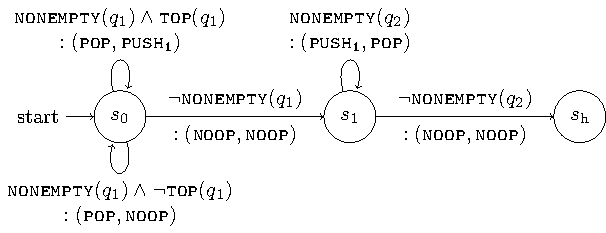
\includegraphics{PDA.pdf}
		\caption{a double-stack PDA computing unary addition}
		\label{fig:PDA}
	\end{figure}
	\begin{table}[t]
	\centering
	\begin{tabular}{|c| c c c |}
		\hline 
		Time & State & Stack 1 & Stack 2 \\
		\hline
		0 & $s_0$ & 101 & $\varepsilon$ \\
		1 & $s_0$ & 01 & 1 \\
		2 & $s_0$ & 1 & 1 \\
		3 & $s_0$ & $\varepsilon$ & 11 \\
		4 & $s_1$ & $\varepsilon$ & 11 \\
		5 & $s_1$ & 1 & 1 \\
		6 & $s_1$ & 11 & $\varepsilon$ \\
		7 & $s_\h$ & 11 & $\varepsilon$ \\
		\hline
	\end{tabular}
	\caption{execution of the double-stack PDA in figure \ref{fig:PDA} with input 101}
	\label{tab:execution}
\end{table}
	\begingroup
	\allowdisplaybreaks
	\begin{align*}
		x_0^+=\sigma\big(&x_0^+\big) \tag{since $x_0^+\in\{0,1\}$} \\
			 =\sigma(&x_0\cdot\nonempty(q_1)\cdot\tos(q_1)\:+ \\
					 &x_0\cdot\nonempty(q_1)\cdot\lnot\tos(q_1)) \\	
			 =\sigma(&\sigma(x_0+\nonempty(q_1)+\tos(q_1)-2)\:+ \\
					 &\sigma(x_0+\nonempty(q_1)+\lnot\tos(q_1)-2)) \tag{by equation \ref{eq:towardsLemmaState}}	\\
			 =\sigma(&\sigma(x_0+\sigma(4q_1)+\sigma(4q_1-2)-2)\:+ \\
					 &\sigma(x_0+\sigma(4q_1)+1-\sigma(q_1-2)-2)) \tag{by equations \ref{eq:top} and \ref{eq:nonempty}}	\\
			 =\sigma(&\underbrace{\sigma(x_0+\sigma(4q_1)+\sigma(4q_1-2)-2)}_\text{$\eqdef\sigma_1$}+ \\
					 &\underbrace{\sigma(x_0+\sigma(4q_1)-\sigma(4q_1-2)-1)}_\text{$\eqdef\sigma_2$}) \\\\
		x_1^+=\sigma\big(&x_1^+\big) \tag{since $x_1^+\in\{0,1\}$} \\
			 =\sigma(&x_0\cdot\lnot\nonempty(q_1)\:+ \\
					 &x_1\cdot\nonempty(q_2)) \\
			 =\sigma(&\sigma(x_0+\lnot\nonempty(q_1)-1)\:+ \\
					 &\sigma(x_1+\nonempty(q_2)-1)) \tag{by equation \ref{eq:towardsLemmaState}} \\
			 =\sigma(&\sigma(x_0+1-\sigma(4q_1)-1)\:+ \\
					 &\sigma(x_1+\sigma(4q_2)-1)) \tag{by equation \ref{eq:nonempty}} \\
			 =\sigma(&\underbrace{\sigma(x_0-\sigma(4q_1))}_\text{$\eqdef\sigma_3$}+ \\
					 &\underbrace{\sigma(x_1+\sigma(4q_2)-1)}_\text{$\eqdef\sigma_4$}) \\\\
		x_\h^+=\sigma\big(&x_\h^+\big) \tag{since $x_\h^+\in\{0,1\}$} \\
			  =\sigma(&x_1\cdot\lnot\nonempty(q_2)) \\
			  =\sigma(&\sigma(x_1+\lnot\nonempty(q_2)-1)) \tag{by equation \ref{eq:towardsLemmaState}}	\\
			  =\sigma(&\sigma(x_1+1-\sigma(4q_2)-1)) \tag{by equation \ref{eq:nonempty}} \\
			  =\sigma(&\underbrace{\sigma(x_1-\sigma(4q_2))}_\text{$\eqdef\sigma_5$}) \\\\
		q_1^+=\sigma\big(&q_1^+\big) \tag{since $q_1^+\in[0,1)$} \\
			 =\sigma(&x_0\cdot\nonempty(q_1)\cdot\tos(q_1)\cdot\pop(q_1)\:+ \\
					 &x_0\cdot\nonempty(q_1)\cdot\lnot\tos(q_1)\cdot\pop(q_1)\:+ \\
					 &x_0\cdot\lnot\nonempty(q_1)\cdot\noop(q_1)\:+ \\
					 &x_1\cdot\nonempty(q_2)\cdot\pushone(q_1)\:+ \\
					 &x_1\cdot\lnot\nonempty(q_2)\cdot\noop(q_1)) \\
			 =\sigma(&\sigma(x_0+\nonempty(q_1)+\tos(q_1)-3+\pop(q_1))\:+ \\
					 &\sigma(x_0+\nonempty(q_1)+\lnot\tos(q_1)-3+\pop(q_1))\:+ \\
					 &\sigma(x_0+\lnot\nonempty(q_1)-2+\noop(q_1))\:+ \\
					 &\sigma(x_1+\nonempty(q_2)-2+\pushone(q_1))\:+ \\
					 &\sigma(x_1+\lnot\nonempty(q_2)-2+\noop(q_1))) \tag{by equation \ref{eq:towardsLemmaState}} \\
			 =\sigma\big(&\sigma(x_0+\sigma(4q_1)+\sigma(4q_1-2)-3+4q_1-2\sigma(4q_1-2)-1)\:+ \\
					 &\sigma(x_0+\sigma(4q_1)+1-\sigma(4q_1-2)-3+4q_1-2\sigma(4q_1-2)-1)\:+ \\
					 &\sigma(x_0+1-\sigma(4q_1)-2+q_1)\:+ \\
					 &\sigma\big(x_1+\sigma(4q_2)-2+\textstyle{\frac{1}{4}}q_1+\textstyle{\frac{3}{4}}\big)\:+ \\
					 &\sigma(x_1+1-\sigma(4q_2)-2+q_1)\big) \tag{by equations \ref{eq:top}, \ref{eq:nonempty}, \ref{eq:push1}, and \ref{eq:pop}} \\
			 =\sigma\big(&\underbrace{\sigma(x_0+\sigma(4q_1)-\sigma(4q_1-2)+4q_1-4)}_\text{$\eqdef\sigma_6$}+ \\
					 &\underbrace{\sigma(x_0+\sigma(4q_1)-3\sigma(4q_1-2)+4q_1-3)}_\text{$\eqdef\sigma_7$}+ \\
					 &\underbrace{\sigma(x_0-\sigma(4q_1)+q_1-1)}_\text{$\eqdef\sigma_8$}+ \\
					 &\underbrace{\sigma\big(x_1+\sigma(4q_2)+\textstyle{\frac{1}{4}}q_1-\textstyle{\frac{5}{4}}\big)}_\text{$\eqdef\sigma_9$}+ \\
					 &\underbrace{\sigma(x_1-\sigma(4q_2)+q_1-1)}_\text{$\eqdef\sigma_{10}$}\big) \\\\
		q_2^+=\sigma\big(&q_2^+\big) \tag{since $q_2^+\in[0,1)$} \\
			 =\sigma(&x_0\cdot\nonempty(q_1)\cdot\tos(q_1)\cdot\pushone(q_2)\:+ \\
					 &x_0\cdot\nonempty(q_1)\cdot\lnot\tos(q_1)\cdot\noop(q_2)\:+ \\
					 &x_0\cdot\lnot\nonempty(q_1)\cdot\noop(q_2)\:+ \\
					 &x_1\cdot\nonempty(q_2)\cdot\pop(q_2)\:+ \\
					 &x_1\cdot\lnot\nonempty(q_2)\cdot\noop(q_2)) \\
			 =\sigma(&\sigma(x_0+\nonempty(q_1)+\tos(q_1)-3+\pushone(q_2))\:+ \\
					 &\sigma(x_0+\nonempty(q_1)+\lnot\tos(q_1)-3+\noop(q_2))\:+ \\
					 &\sigma(x_0+\lnot\nonempty(q_1)-2+\noop(q_2))\:+ \\
					 &\sigma(x_1+\nonempty(q_2)-2+\pop(q_2))\:+ \\
					 &\sigma(x_1+\lnot\nonempty(q_2)-2+\noop(q_2))) \tag{by equation \ref{eq:towardsLemmaState}} \\
			 =\sigma\big(&\sigma\big(x_0+\sigma(4q_1)+\sigma(4q_1-2)-3+\textstyle{\frac{1}{4}}q_2+\textstyle{\frac{3}{4}}\big)\:+ \\
					 &\sigma(x_0+\sigma(4q_1)+1-\sigma(4q_1-2)-3+q_2)\:+ \\
					 &\sigma(x_0+1-\sigma(4q_1)-2+q_2)\:+ \\
					 &\sigma(x_1+\sigma(4q_2)-2+4q_2-2\sigma(4q_2-2)-1)\:+ \\
					 &\sigma(x_1+1-\sigma(4q_2)-2+q_2)\big) \tag{by equations \ref{eq:top}, \ref{eq:nonempty}, \ref{eq:push1}, and \ref{eq:pop}} \\
			 =\sigma\big(&\underbrace{\sigma\big(x_0+\sigma(4q_1)-\sigma(4q_1-2)+\textstyle{\frac{1}{4}}q_2-\textstyle{\frac{9}{4}}\big)}_\text{$\eqdef\sigma_{11}$}+ \\
					 &\underbrace{\sigma(x_0+\sigma(4q_1)-\sigma(4q_1-2)+q_2-2)}_\text{$\eqdef\sigma_{12}$}+ \\
					 &\underbrace{\sigma(x_0-\sigma(4q_1)+q_2-1)}_\text{$\eqdef\sigma_{13}$}+ \\
					 &\underbrace{\sigma(x_1+\sigma(4q_2)-2\sigma(4q_2-2)+4q_2-3)}_\text{$\eqdef\sigma_{14}$}+ \\
					 &\underbrace{\sigma(x_1-\sigma(4q_2)+q_2-1)}_\text{$\eqdef\sigma_{15}$}\big).
	\end{align*}
	\endgroup
	
	The neural network $\mathcal{N}$ simulating $\mathcal{M}$ is shown in figure \ref{fig:exampleNet}. 
	\begin{figure}[p]
		\centering
		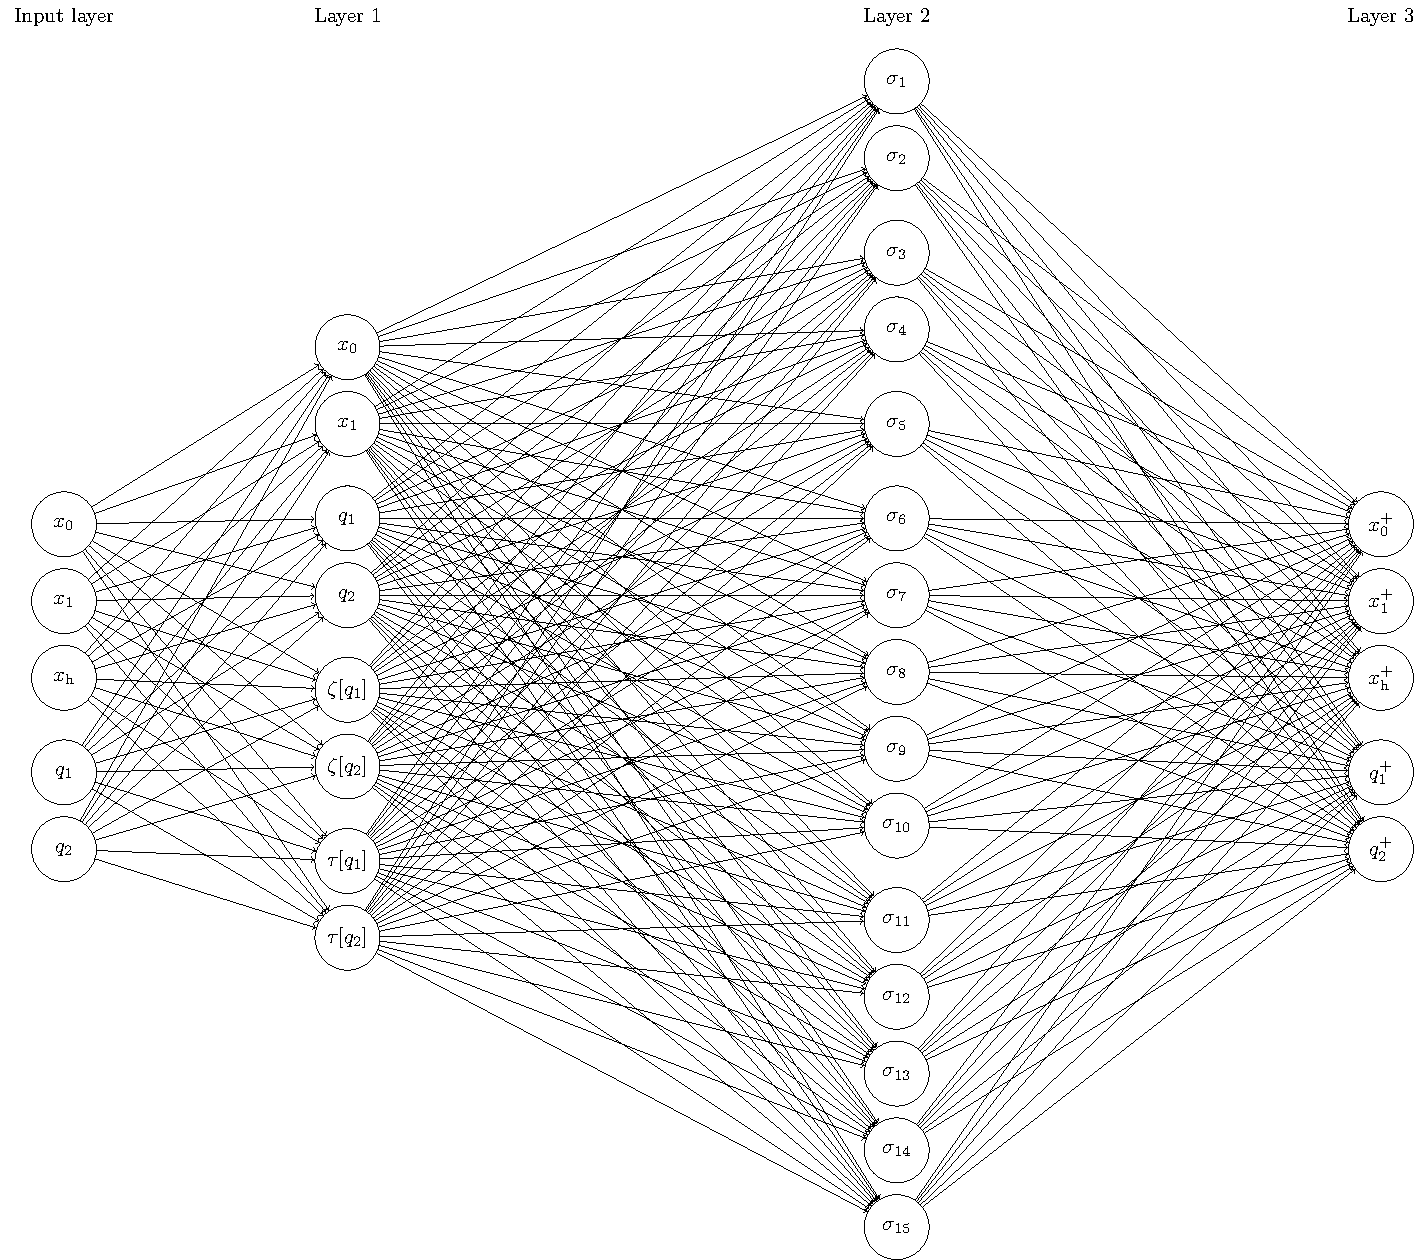
\includegraphics[width=\textwidth]{exampleNet.pdf}
		\caption{a recurrent neural network simulating the double-stack PDA in figure \ref{fig:PDA}}
		\label{fig:exampleNet}
	\end{figure}
	As we already pointed out in corollary \ref{theo:secondSimulation}, the output of $\mathcal{N}$ becomes its own input until $\mathcal{M}$ reaches the halting state, i.e. until the third neuron of the output layer of $\mathcal{N}$ has activation equal to one. When that happens, the activation of the fourth neuron of the output layer will be the encoded output of $\mathcal{M}$, that is, the rational number corresponding to the sum of the two unary numbers in input to $\mathcal{M}$ itself. The weight matrices and bias vectors of $\mathcal{N}$ are shown in tables \ref{tab:W1b1ex}, \ref{tab:W2b2ex}, and \ref{tab:W3b3ex}, where we adopt the more compact notation $\tos(q)\eqdef\zeta[q], \nonempty(q)\eqdef\tau[q]$ introduced in definition \ref{def:topAndNonempty}.
	\begin{table}[p]
	\centering
	\begin{tabular}{|c| c c c c c |c|}
		\hline 
		$W^1$ & $x_0$ & $x_1$ & $x_\h$ & $q_1$ & $q_2$ & $b^1$ \\
		\hline
		$x_0$ & 1 & 0 & 0 & 0 & 0 & 0 \\
		$x_1$ & 0 & 1 & 0 & 0 & 0 & 0 \\
		$q_1$ & 0 & 0 & 0 & 1 & 0 & 0 \\
		$q_2$ & 0 & 0 & 0 & 0 & 1 & 0 \\
		$\zeta[q_1]$ & 0 & 0 & 0 & 4 & 0 & $-2$ \\
		$\zeta[q_2]$ & 0 & 0 & 0 & 0 & 4 & $-2$ \\
		$\tau[q_1]$ & 0 & 0 & 0 & 4 & 0 & 0 \\
		$\tau[q_2]$ & 0 & 0 & 0 & 0 & 4 & 0 \\
		\hline
	\end{tabular}
	\caption{weights from the input layer to layer 1 and biases of layer 1}
	\label{tab:W1b1ex}
\end{table}
	\begin{table}[p]
	\centering
	\begin{tabular}{|c| c c c c c c c c |c|}
		\hline 
		$W^2$ & $x_0$ & $x_1$ & $q_1$ & $q_2$ & $\zeta[q_1]$ & $\zeta[q_2]$ & $\tau[q_1]$ & $\tau[q_2]$ & $b^2$ \\
		\hline
		$\sigma_1$ & 1 & 0 & 0 & 0 & 1 & 0 & 1 & 0 & $-2$ \\
		$\sigma_2$ & 1 & 0 & 0 & 0 & $-1$ & 0 & 1 & 0 & $-1$ \\
		$\sigma_3$ & 1 & 0 & 0 & 0 & 0 & 0 & $-1$ & 0 & 0 \\
		$\sigma_4$ & 0 & 1 & 0 & 0 & 0 & 0 & 0 & 1 & $-1$ \\
		$\sigma_5$ & 0 & 1 & 0 & 0 & 0 & 0 & 0 & $-1$ & 0 \\
		$\sigma_6$ & 1 & 0 & 4 & 0 & $-1$ & 0 & 1 & 0 & $-4$ \\
		$\sigma_7$ & 1 & 0 & 4 & 0 & $-3$ & 0 & 1 & 0 & $-3$ \\
		$\sigma_8$ & 1 & 0 & 1 & 0 & 0 & 0 & $-1$ & 0 & $-1$ \\
		$\sigma_9$ & 0 & 1 & $\frac{1}{4}$ & 0 & 0 & 0 & 0 & 1 & $-\frac{5}{4}$ \\
		$\sigma_{10}$ & 0 & 1 & 1 & 0 & 0 & 0 & 0 & $-1$ & $-1$ \\
		$\sigma_{11}$ & 1 & 0 & 0 & $\frac{1}{4}$ & 1 & 0 & 1 & 0 & $-\frac{9}{4}$ \\
		$\sigma_{12}$ & 1 & 0 & 0 & 1 & $-1$ & 0 & 1 & 0 & $-2$ \\
		$\sigma_{13}$ & 1 & 0 & 0 & 1 & 0 & 0 & $-1$ & 0 & $-1$ \\
		$\sigma_{14}$ & 0 & 1 & 0 & 4 & 0 & $-2$ & 0 & 1 & $-3$ \\
		$\sigma_{15}$ & 0 & 1 & 0 & 1 & 0 & 0 & 0 & $-1$ & $-1$ \\
		\hline
	\end{tabular}
	\caption{weights from layer 1 to layer 2 and biases of layer 2}
	\label{tab:W2b2ex}
\end{table}
	\begin{table}[p]
	\centering
	\begin{tabular}{|c| c c c c c c c c c c c c c c c |c|}
		\hline 
		$W^3$ & $\sigma_1$ & $\sigma_2$ & $\sigma_3$ & $\sigma_4$ & $\sigma_5$ & $\sigma_6$ & $\sigma_7$ & $\sigma_8$ & $\sigma_9$ &  $\sigma_{10}$ & $\sigma_{11}$ & $\sigma_{12}$ & $\sigma_{13}$ & $\sigma_{14}$ & $\sigma_{15}$ & $b^3$ \\
		\hline
		$x_0^+$ & 1 & 1 & 0 & 0 & 0 & 0 & 0 & 0 & 0 & 0 & 0 & 0 & 0 & 0 & 0 & 0 \\
		$x_1^+$ & 0 & 0 & 1 & 1 & 0 & 0 & 0 & 0 & 0 & 0 & 0 & 0 & 0 & 0 & 0 & 0 \\
		$x_\h^+$ & 0 & 0 & 0 & 0 & 1 & 0 & 0 & 0 & 0 & 0 & 0 & 0 & 0 & 0 & 0 & 0 \\
		$q_1^+$ & 0 & 0 & 0 & 0 & 0 & 1 & 1 & 1 & 1 & 1 & 0 & 0 & 0 & 0 & 0 & 0 \\
		$q_2^+$ & 0 & 0 & 0 & 0 & 0 & 0 & 0 & 0 & 0 & 0 & 1 & 1 & 1 & 1 & 1 & 0 \\
		\hline
	\end{tabular}
	\caption{weights from layer 2 to layer 3 and biases of layer 3}
	\label{tab:W3b3ex}
\end{table}
	
	\section{Implementation}
	The results of section \ref{sec:mathex} can be deployed to obtain an ad hoc implementation of the example we are discussing, allowing us to verify the correctness of our simulation in a simple but representative specific scenario. The code we are going to present is written in Python 3.7. 
	
	First of all, we need a class modeling a stack whose content is encoded as a rational number (see equation \ref{eq:encoding}) and whose operations are defined as in equations \ref{eq:push0}, \ref{eq:push1}, \ref{eq:pop}, and \ref{eq:topAndNonempty}:
	\begin{verbatim}
		"""
		stack.py
		~~~~~~~~
		"""

		class Stack:

		    def __init__(self, stack):
			    """stack must be a list of binary values representing, 
			    from left to right, the stack content from top to bottom."""
		        self.encoding = 0
		        for i in range(len(stack)):
		            self.encoding += (2 * stack[i] + 1) / 4 ** (i + 1)

		    def top(self):
		        return self.encoding > 0.5

		    def nonempty(self):
		        return self.encoding != 0

		    def push(self, symbol):
		        if symbol != 0 and symbol != 1:
		            raise ValueError('Stack symbols must be binary')
		        self.encoding = self.encoding / 4 + (2 * symbol + 1) / 4

		    def pop(self):
		        if not self.nonempty():
		            raise RuntimeError('Cannot pop an empty stack')
		        self.encoding = 4 * self.encoding - 2 * self.top() - 1
	\end{verbatim}
	Then, we write a class defining the double-stack PDA in figure \ref{fig:PDA}:
	\begin{verbatim}
		"""
		machine.py
		~~~~~~~~~~
		"""
		
		from stack import Stack
		
		class DoubleStackPDA:
		
		    def __init__(self, stack1):
		        """stack1 must be a list containing the two 
		        unary numbers to add separated by a zero."""
		        self.stack1 = Stack(stack1)
		        self.stack2 = Stack([])
		        self.states = ['s0', 's1', 'sh']
		        self.state = self.states[0]
		
		    def update(self):
		        if self.state is self.states[0] and \
		                self.stack1.nonempty() and \
		                self.stack1.top():
		            self.stack1.pop()
		            self.stack2.push(1)
		        elif self.state is self.states[0] and \
		                self.stack1.nonempty() and \ 
		                not self.stack1.top():
		            self.stack1.pop()
		        elif self.state is self.states[0] and \
		                not self.stack1.nonempty():
		            self.state = self.states[1]
		        elif self.state is self.states[1] and \ 
		                self.stack2.nonempty():
		            self.stack1.push(1)
		            self.stack2.pop()
		        elif self.state is self.states[1] and \
		                not self.stack2.nonempty():
		            self.state = self.states[2]
		        else:
		            raise RuntimeError('Undefined transition')
		
		    def execute(self):
		        while self.state is not self.states[2]:
		            self.update()
		        print('Stack 1 encoding = {}'.format(self.stack1.encoding))
		        print('Stack 2 encoding = {}'.format(self.stack2.encoding))
	\end{verbatim}
	Furthermore, by using tables \ref{tab:W1b1ex}, \ref{tab:W2b2ex}, and \ref{tab:W3b3ex}, we can implement the neural network in figure \ref{fig:exampleNet} (the following code is loosely inspired by \cite{nets}):
	\begin{verbatim}
		"""
		network.py
		~~~~~~~~~~
		"""
		
		import numpy
		from stack import Stack
		
		class Network:
		
		    def __init__(self):
		        self.weights = [
		            numpy.array([[1, 0, 0, 0, 0],
		                         [0, 1, 0, 0, 0],
		                         [0, 0, 0, 1, 0],
		                         [0, 0, 0, 0, 1],
		                         [0, 0, 0, 4, 0],
		                         [0, 0, 0, 0, 4],
		                         [0, 0, 0, 4, 0],
		                         [0, 0, 0, 0, 4]]),
		            numpy.array([[1, 0, 0, 0, 1, 0, 1, 0],
		                         [1, 0, 0, 0, -1, 0, 1, 0],
		                         [1, 0, 0, 0, 0, 0, -1, 0],
		                         [0, 1, 0, 0, 0, 0, 0, 1],
		                         [0, 1, 0, 0, 0, 0, 0, -1],
		                         [1, 0, 4, 0, -1, 0, 1, 0],
		                         [1, 0, 4, 0, -3, 0, 1, 0],
		                         [1, 0, 1, 0, 0, 0, -1, 0],
		                         [0, 1, 1/4, 0, 0, 0, 0, 1],
		                         [0, 1, 1, 0, 0, 0, 0, -1],
		                         [1, 0, 0, 1/4, 1, 0, 1, 0],
		                         [1, 0, 0, 1, -1, 0, 1, 0],
		                         [1, 0, 0, 1, 0, 0, -1, 0],
		                         [0, 1, 0, 4, 0, -2, 0, 1],
		                         [0, 1, 0, 1, 0, 0, 0, -1]]),
		            numpy.array([[1, 1, 0, 0, 0, 0, 0, 0, 0, 0, 0, 0, 0, 0, 0],
		                         [0, 0, 1, 1, 0, 0, 0, 0, 0, 0, 0, 0, 0, 0, 0],
		                         [0, 0, 0, 0, 1, 0, 0, 0, 0, 0, 0, 0, 0, 0, 0],
		                         [0, 0, 0, 0, 0, 1, 1, 1, 1, 1, 0, 0, 0, 0, 0],
		                         [0, 0, 0, 0, 0, 0, 0, 0, 0, 0, 1, 1, 1, 1, 1]])
		        ]
		        self.biases = [
		            numpy.array([0, 0, 0, 0, -2, -2, 0, 0]),
		            numpy.array([-2, -1, 0, -1, 0, -4, -3, 
		                         -1, -5/4, -1, -9/4, -2, -1, -3, -1]),
		            numpy.zeros(5)
		        ]
		
		    def execute(self, stack1):
		    
		        def feedforward(a):
		            if a[2] == 1:
		                return a[3], a[4]
		            for w, b in zip(self.weights, self.biases):
		                a = sigmoid(numpy.dot(w, a) + b)
		            return feedforward(a)
		    
		        a = numpy.array(
		            [1, 0, 0, Stack(stack1).encoding, Stack([]).encoding]
		        )
		        stack1_encoding, stack2_encoding = feedforward(a)
		        print('Stack 1 encoding = {}'.format(stack1_encoding))
		        print('Stack 2 encoding = {}'.format(stack2_encoding))
		
		def sigmoid(x):
		    """Applies the sigmoid function elementwise."""
		    return numpy.piecewise(
		        x, 
		        [x < 0, numpy.logical_and(0 <= x, x <= 1), x > 1], 
		        [0, lambda x: x, 1]
		    )
	\end{verbatim}
	Finally, we write a test to see if the simulation actually works:
	\begin{verbatim}
		"""
		test.py
		~~~~~~~
		"""
		
		from machine import DoubleStackPDA
		from network import Network
		
		stack = [1, 0, 1]
		
		print('\n======== Double-stack PDA ========\n')
		m = DoubleStackPDA(stack)
		m.execute()
		
		print('\n======== Neural network ========\n')
		n = Network()
		n.execute(stack)
	\end{verbatim}
	and, if we run such test, we get	
	\begin{verbatim}
		======== Double-stack PDA ========
		
		Stack 1 encoding = 0.9375
		Stack 2 encoding = 0.0
		
		======== Neural network ========
		
		Stack 1 encoding = 0.9375
		Stack 2 encoding = 0.0
	\end{verbatim}
	which shows that the neural network correctly simulates the double-stack PDA.
	
	\begin{thebibliography}{9}
		\bibitem{SiegSon}
			Hava T. Siegelmann, Eduardo D. Sontag.
			\textquotedblleft On the Computational Power of Neural Nets\textquotedblright.
			In \textit{Proceedings of the fifth Annual ACM Workshop on Computational Learning Theory} (COLT 1992), pp. 440--449.
			\textsc{doi}: \texttt{10.1145/130385.130432}. 
			\textsc{url}: \url{http://binds.cs.umass.edu/papers/1992_Siegelmann_COLT.pdf}
		\bibitem{nets}
			Michael A. Nielsen. 
			\textit{Neural Networks and Deep Learning}. 
			Determination Press, 2015.
			\textsc{url}: \url{http://neuralnetworksanddeeplearning.com}
		\bibitem{slides}
			Benjamin Wilson.
			\textit{Siegelmann \& Sontag's \textquotedblleft On the Computational Power of Neural Nets\textquotedblright}.
			 From a talk given at the Sydney Machine Learning Meetup, 2018. 
			 \textsc{url}: \url{http://drive.google.com/file/d/1HR-dXSI-dX16yibiXeeiz4pP2D8_KYDl/view}
	\end{thebibliography}
	
\end{document}